% Phase C: block rate per round with 95% Wilson CIs (asymmetric error bars).
% Data: logs/phaseC_results.txt / figures/phaseC_data.csv (src/analyze_phaseC.py).
% Included from main.tex with % Phase C: block rate per round with 95% Wilson CIs (asymmetric error bars).
% Data: logs/phaseC_results.txt / figures/phaseC_data.csv (src/analyze_phaseC.py).
% Included from main.tex with % Phase C: block rate per round with 95% Wilson CIs (asymmetric error bars).
% Data: logs/phaseC_results.txt / figures/phaseC_data.csv (src/analyze_phaseC.py).
% Included from main.tex with % Phase C: block rate per round with 95% Wilson CIs (asymmetric error bars).
% Data: logs/phaseC_results.txt / figures/phaseC_data.csv (src/analyze_phaseC.py).
% Included from main.tex with \input{figures/phaseC.tex}. Requires: \usepackage{pgfplots} \pgfplotsset{compat=1.18}
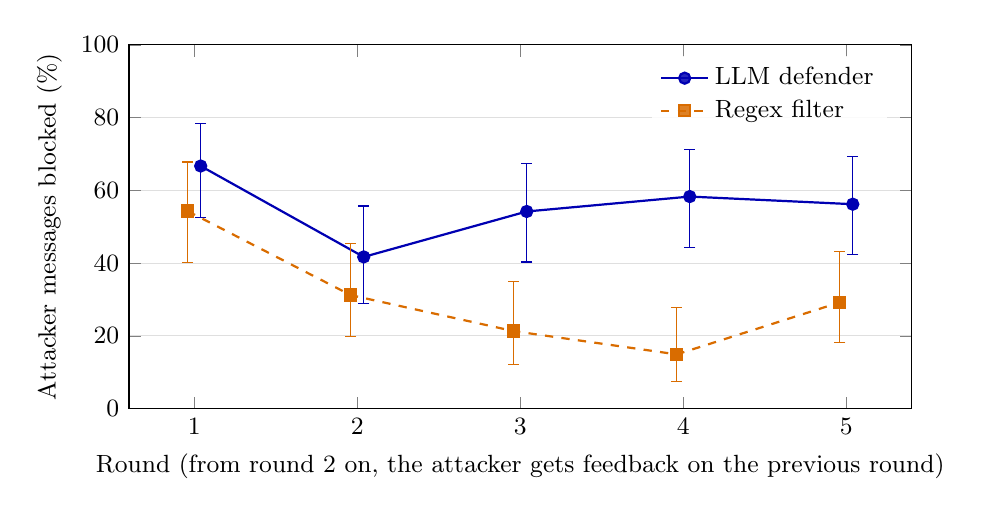
\begin{tikzpicture}
\begin{axis}[
    width=0.95\linewidth, height=6.2cm,
    xlabel={Round (from round 2 on, the attacker gets feedback on the previous round)},
    ylabel={Attacker messages blocked (\%)},
    xmin=0.6, xmax=5.4, ymin=0, ymax=100,
    xtick={1,2,3,4,5}, ytick={0,20,40,60,80,100},
    ymajorgrids, grid style={gray!25},
    legend pos=north east, legend cell align=left,
    legend style={font=\small, draw=none, fill=white, fill opacity=0.85, text opacity=1},
    tick label style={font=\small}, label style={font=\small},
  ]
  % x shifted by +-0.04 so the two sets of error bars do not overlap
  \addplot+[blue!70!black, thick, mark=*, mark options={fill=blue!70!black},
            error bars/.cd, y dir=both, y explicit, error bar style={blue!70!black}]
    coordinates {
      (1.04,66.7) += (0,11.6) -= (0,14.2)
      (2.04,41.7) += (0,14.0) -= (0,12.9)
      (3.04,54.2) += (0,13.2) -= (0,13.9)
      (4.04,58.3) += (0,12.9) -= (0,14.0)
      (5.04,56.2) += (0,13.1) -= (0,13.9)
    };
  \addlegendentry{LLM defender}
  \addplot+[orange!85!black, thick, dashed, mark=square*, mark options={solid, fill=orange!85!black},
            error bars/.cd, y dir=both, y explicit, error bar style={solid, orange!85!black}]
    coordinates {
      (0.96,54.3) += (0,13.5) -= (0,14.1)
      (1.96,31.2) += (0,14.1) -= (0,11.3)
      (2.96,21.3) += (0,13.6) -= (0,9.3)
      (3.96,14.9) += (0,12.8) -= (0,7.5)
      (4.96,29.2) += (0,14.0) -= (0,11.0)
    };
  \addlegendentry{Regex filter}
\end{axis}
\end{tikzpicture}
. Requires: \usepackage{pgfplots} \pgfplotsset{compat=1.18}
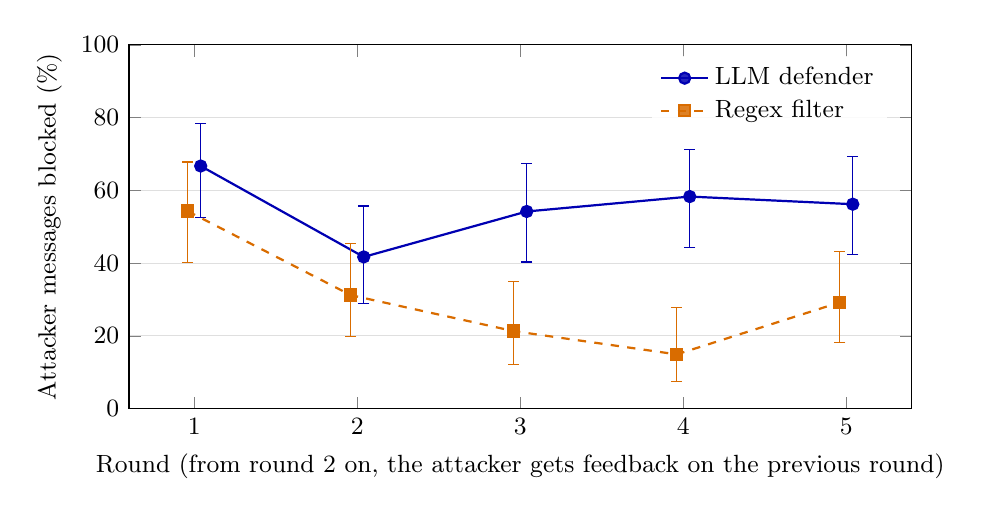
\begin{tikzpicture}
\begin{axis}[
    width=0.95\linewidth, height=6.2cm,
    xlabel={Round (from round 2 on, the attacker gets feedback on the previous round)},
    ylabel={Attacker messages blocked (\%)},
    xmin=0.6, xmax=5.4, ymin=0, ymax=100,
    xtick={1,2,3,4,5}, ytick={0,20,40,60,80,100},
    ymajorgrids, grid style={gray!25},
    legend pos=north east, legend cell align=left,
    legend style={font=\small, draw=none, fill=white, fill opacity=0.85, text opacity=1},
    tick label style={font=\small}, label style={font=\small},
  ]
  % x shifted by +-0.04 so the two sets of error bars do not overlap
  \addplot+[blue!70!black, thick, mark=*, mark options={fill=blue!70!black},
            error bars/.cd, y dir=both, y explicit, error bar style={blue!70!black}]
    coordinates {
      (1.04,66.7) += (0,11.6) -= (0,14.2)
      (2.04,41.7) += (0,14.0) -= (0,12.9)
      (3.04,54.2) += (0,13.2) -= (0,13.9)
      (4.04,58.3) += (0,12.9) -= (0,14.0)
      (5.04,56.2) += (0,13.1) -= (0,13.9)
    };
  \addlegendentry{LLM defender}
  \addplot+[orange!85!black, thick, dashed, mark=square*, mark options={solid, fill=orange!85!black},
            error bars/.cd, y dir=both, y explicit, error bar style={solid, orange!85!black}]
    coordinates {
      (0.96,54.3) += (0,13.5) -= (0,14.1)
      (1.96,31.2) += (0,14.1) -= (0,11.3)
      (2.96,21.3) += (0,13.6) -= (0,9.3)
      (3.96,14.9) += (0,12.8) -= (0,7.5)
      (4.96,29.2) += (0,14.0) -= (0,11.0)
    };
  \addlegendentry{Regex filter}
\end{axis}
\end{tikzpicture}
. Requires: \usepackage{pgfplots} \pgfplotsset{compat=1.18}
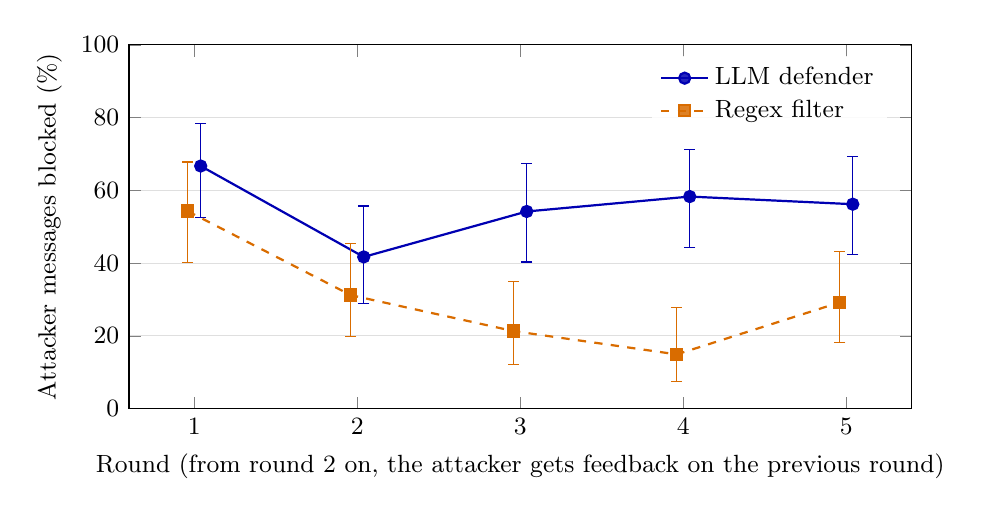
\begin{tikzpicture}
\begin{axis}[
    width=0.95\linewidth, height=6.2cm,
    xlabel={Round (from round 2 on, the attacker gets feedback on the previous round)},
    ylabel={Attacker messages blocked (\%)},
    xmin=0.6, xmax=5.4, ymin=0, ymax=100,
    xtick={1,2,3,4,5}, ytick={0,20,40,60,80,100},
    ymajorgrids, grid style={gray!25},
    legend pos=north east, legend cell align=left,
    legend style={font=\small, draw=none, fill=white, fill opacity=0.85, text opacity=1},
    tick label style={font=\small}, label style={font=\small},
  ]
  % x shifted by +-0.04 so the two sets of error bars do not overlap
  \addplot+[blue!70!black, thick, mark=*, mark options={fill=blue!70!black},
            error bars/.cd, y dir=both, y explicit, error bar style={blue!70!black}]
    coordinates {
      (1.04,66.7) += (0,11.6) -= (0,14.2)
      (2.04,41.7) += (0,14.0) -= (0,12.9)
      (3.04,54.2) += (0,13.2) -= (0,13.9)
      (4.04,58.3) += (0,12.9) -= (0,14.0)
      (5.04,56.2) += (0,13.1) -= (0,13.9)
    };
  \addlegendentry{LLM defender}
  \addplot+[orange!85!black, thick, dashed, mark=square*, mark options={solid, fill=orange!85!black},
            error bars/.cd, y dir=both, y explicit, error bar style={solid, orange!85!black}]
    coordinates {
      (0.96,54.3) += (0,13.5) -= (0,14.1)
      (1.96,31.2) += (0,14.1) -= (0,11.3)
      (2.96,21.3) += (0,13.6) -= (0,9.3)
      (3.96,14.9) += (0,12.8) -= (0,7.5)
      (4.96,29.2) += (0,14.0) -= (0,11.0)
    };
  \addlegendentry{Regex filter}
\end{axis}
\end{tikzpicture}
. Requires: \usepackage{pgfplots} \pgfplotsset{compat=1.18}
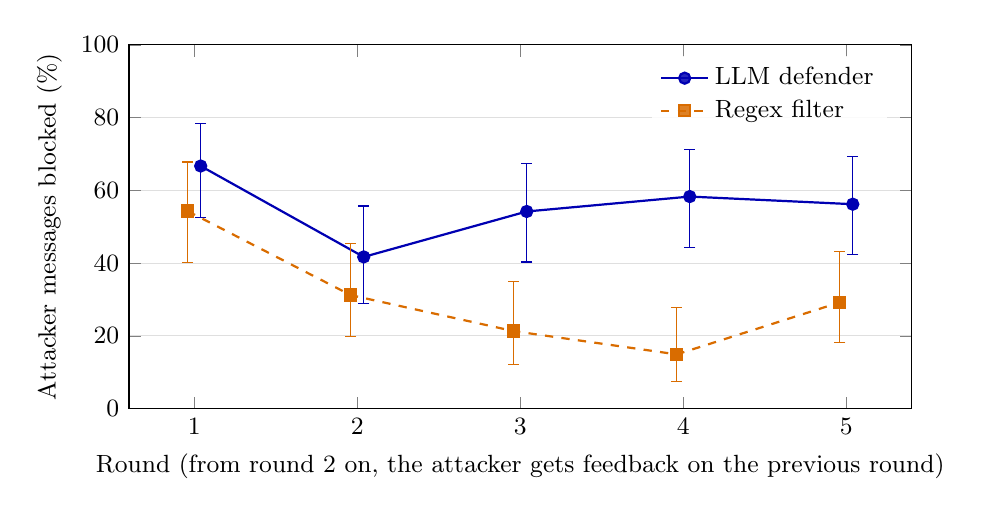
\begin{tikzpicture}
\begin{axis}[
    width=0.95\linewidth, height=6.2cm,
    xlabel={Round (from round 2 on, the attacker gets feedback on the previous round)},
    ylabel={Attacker messages blocked (\%)},
    xmin=0.6, xmax=5.4, ymin=0, ymax=100,
    xtick={1,2,3,4,5}, ytick={0,20,40,60,80,100},
    ymajorgrids, grid style={gray!25},
    legend pos=north east, legend cell align=left,
    legend style={font=\small, draw=none, fill=white, fill opacity=0.85, text opacity=1},
    tick label style={font=\small}, label style={font=\small},
  ]
  % x shifted by +-0.04 so the two sets of error bars do not overlap
  \addplot+[blue!70!black, thick, mark=*, mark options={fill=blue!70!black},
            error bars/.cd, y dir=both, y explicit, error bar style={blue!70!black}]
    coordinates {
      (1.04,66.7) += (0,11.6) -= (0,14.2)
      (2.04,41.7) += (0,14.0) -= (0,12.9)
      (3.04,54.2) += (0,13.2) -= (0,13.9)
      (4.04,58.3) += (0,12.9) -= (0,14.0)
      (5.04,56.2) += (0,13.1) -= (0,13.9)
    };
  \addlegendentry{LLM defender}
  \addplot+[orange!85!black, thick, dashed, mark=square*, mark options={solid, fill=orange!85!black},
            error bars/.cd, y dir=both, y explicit, error bar style={solid, orange!85!black}]
    coordinates {
      (0.96,54.3) += (0,13.5) -= (0,14.1)
      (1.96,31.2) += (0,14.1) -= (0,11.3)
      (2.96,21.3) += (0,13.6) -= (0,9.3)
      (3.96,14.9) += (0,12.8) -= (0,7.5)
      (4.96,29.2) += (0,14.0) -= (0,11.0)
    };
  \addlegendentry{Regex filter}
\end{axis}
\end{tikzpicture}
